\chapter{Introduction}
% Change page numbers back to Arabic numerals and reset the page count
\renewcommand{\thepage}{\arabic{page}}
\setcounter{page}{1}

As shown in Figure \ref{intro}, two robots perform a competition in this project. One robot chase the other and try to hit the opponent with laser. And the other robot tries to hide from the laser. Both robots are controlled via intelligent algorithms. This report mainly introduces the algorithms for image processing, hiding and attacking strategies, path planning and robot control.

\begin{figure}[thb]
    \centering
    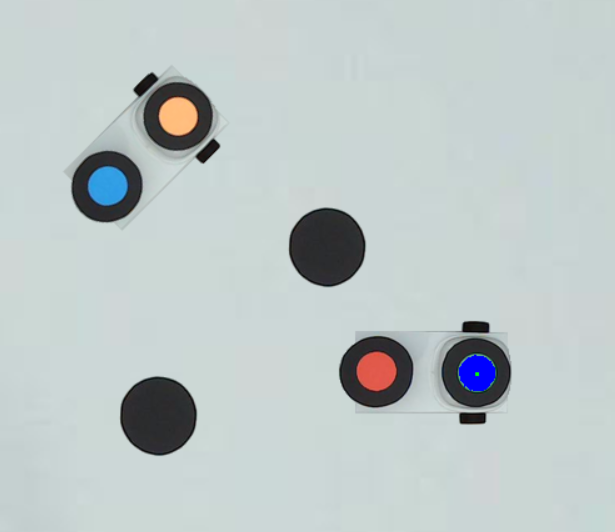
\includegraphics[width=0.5\textwidth]{images/intro.png}
    \caption[Overview of the project]{Overview of the project.}\label{intro}
\end{figure}

\section{Modelling of the Robot}

In order to simplify the robot model, we assume that there is no wheel slipping. And the basic structure of robot is shown in Figure \ref{vehicle_model}.

\begin{figure}[thb]
    \centering
    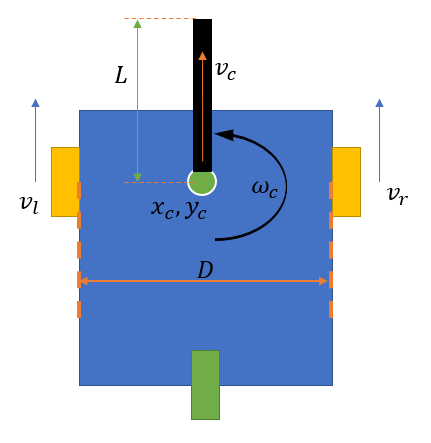
\includegraphics[width=0.5\textwidth]{images/vehicle_model.png}
    \caption[vehicle model]{vehicle model.}\label{vehicle_model}
\end{figure}

$$ v_r = \omega_r R $$

Where $v_r$ is the linear velocity, $R$ is the radius of wheel, and $\omega_r$ is the angular velocity.

\begin{figure}[thb]
    \centering
    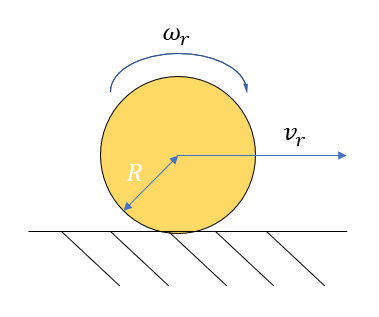
\includegraphics[width=0.5\textwidth]{images/wheel_model.png}
    \caption[wheel model]{wheel model.}\label{intro}
\end{figure}

$x_c$ and $y_c$ is the coordinate of the vehicle centre. $\theta$ is the direction of vehicle. $D$ is the distance bewteen two wheels. The geometry model of this vehicle is shown below:

$$ v_c = (v_r+v_l)/2 $$
$$ \omega_c = ( v_r - v_l ) / D $$
$$ \dot{\theta_c} = \omega_c = ( v_r - v_l ) / D $$

\section{System Structure}

The flowchart of the whole system is shown in Figure \ref{system_flow}

\begin{figure}[thb]
    \centering
    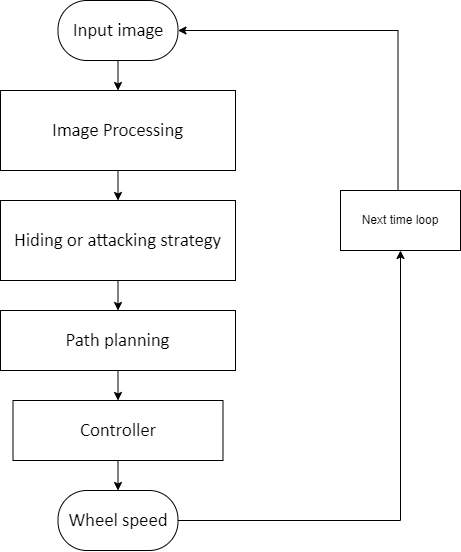
\includegraphics[width=0.8\textwidth]{images/system_flow.png}
    \caption[the flowchart of the whole system]{the flowchart of the whole system.}\label{system_flow}
\end{figure}

The input and output for each part is shown in Table \ref{system_io}. The input of subsequent part is the output of last part.

\begin{table}[h]\footnotesize
\begin{tabular}{c|cc}
    \hline 
    Part&Input&Output\\
    \hline 
    Image processing&RGB image of the whole map&\makecell[c]{Positions of every object\\ with identification}\\
    \hline 
    Hiding Strategy&output from image processing&expected hiding position\\
    \hline 
    Attacking strategy&output from image processing&\makecell[c]{expected attacking\\ position and fire order}\\
    \hline 
    Path planning &\makecell[c]{current position and \\expected position}& \makecell[c]{expected trajectory avoiding \\the obstacles and boundary of map}\\
    \hline 
    Controller &next point of expected trajectory&speed of two wheels\\
    \hline 
\end{tabular}
\caption[the input and output for each part in system]{the input and output for each part in system.}\label{system_io}
\end{table}

\section{Teamwork}

The job of every team member is shown in table \ref{teamwork}.

\begin{table}[htbp]\footnotesize
\addtolength{\leftskip} {-1.5cm}
\begin{tabular}{c|cccc}
\hline 
Name&Qiaomeng Qin&Xiaobo Wu&Yuelong Wu&Mario\\
\hline 
Project Management&System design&&&  \\
\hline 
Image Processing&\makecell[c]{Methodology\\Implementation}& & &\\
\hline 
Hiding Strategy&\makecell[c]{Methodology\\Implementation}&Methodology& &Methodology\\
\hline 
Attacking strategy& & & &\makecell[c]{Methodology\\Implementation}\\
\hline 
Path planning& &\makecell[c]{Methodology\\Implementation}& &\\
\hline 
Robot Controller& & & &\makecell[c]{Methodology\\Implementation}\\
\hline 
Report Writing&\makecell[c]{Introduction\\Image Processing\\Hiding Strategy}&\makecell[c]{Hiding Strategy\\Path Planning}&\makecell[c]{Controller Designing\\Attacking Strategy}&\makecell[c]{Controller Designing\\Attacking Strategy}\\
\hline 
\end{tabular}
\caption[the work for each team member]{the work for each team member.}\label{teamwork}
\end{table}


